\documentclass[12pt,oneside]{exam}

% This package simply sets the margins to be 1 inch.
\usepackage[margin=1in]{geometry}

% These packages include nice commands from AMS-LaTeX
\usepackage{amssymb,amsmath,amsthm,amsfonts,latexsym,verbatim,xspace,setspace}
\usepackage{hyperref}
\usepackage{graphicx}

% Make the space between lines slightly more
% generous than normal single spacing, but compensate
% so that the spacing between rows of matrices still
% looks normal.  Note that 1.1=1/.9090909...
\renewcommand{\baselinestretch}{1.1}
\renewcommand{\arraystretch}{.91}

% Define environments for exercises.
\newenvironment{exercise}[1]{\vspace{.1in}\noindent\textbf{Exercise #1 \hspace{.05em}}}{}
\newenvironment{newsolution}{\vspace{.1in}\noindent\textbf{Solution: \hspace{.05em}}}{}

% define shortcut commands for commonly used symbols
\newcommand{\R}{\mathbb{R}}
\newcommand{\C}{\mathbb{C}}
\newcommand{\Z}{\mathbb{Z}}
\newcommand{\Q}{\mathbb{Q}}
\newcommand{\N}{\mathbb{N}}
\newcommand{\calP}{\mathcal{P}}
\DeclareMathOperator{\sech}{sech}
\DeclareMathOperator{\csch}{csch}
\DeclareMathOperator{\vsspan}{span}

\title{Math 203 - Summer I 2020: Solutions to Homework 3}

%%%%%%%%%%%%%%%%%%%%%%%%%%%%%%%%%%%%%%%%%%

\begin{document}

\begin{flushright}
\sc MAT 203 - Summer I 2020\\
June 23, 2020
\end{flushright}
\bigskip
 
\begin{center}
\textsf{Homework 3 solutions} 
\end{center}

%%%%%%%%%%%%%%%%%%%%%%%%%%%%%%%%%%%%%%%%

\begin{exercise}{1}
Find the directional derivative of the function
\begin{equation*}
f(x,y)= \frac{y^2}{4} - x^2,
\end{equation*}
at the point $P=(1,4)$, in the direction of
\begin{equation*}
v = 2\mathbf{i} + \mathbf{j}.
\end{equation*}
\end{exercise}

\begin{newsolution} 
We will compute this directional derivative straight from the definition, as a limit:
\begin{align*}
\frac{\partial f}{\partial v} (1,4) & = \lim_{t \to 0} \frac{ f((1,4)+tv)-f(1,4)}{t} \\
& =\lim_{t \to 0} \frac{ f(1+2t,4+t)-f(1,4)}{t}\\
& = \lim_{t \to 0} \frac{ \frac{(4+t)^2}{4} - (1+2t)^2-\frac{4^2}{4}+1^2}{t}\\
& = \lim_{t \to 0} \frac{16+8t+t^2-4-16t-16t^2-4+1}{4t}\\
& = \lim_{t \to 0} \frac{9-8t-15t^2}{4t} \\
& = -2.
\end{align*}
\end{newsolution}

\begin{exercise}{2}
Use the gradient to function the directional derivative of the function
\begin{equation*}
w = 5x^2 + 2xy -3y^2z
\end{equation*}
at $P=(1,0,1)$, in the direction of
\begin{equation*}
v = \mathbf{i} + \mathbf{j} - \mathbf{k}.
\end{equation*}
\end{exercise}

\begin{newsolution}
The partial derivatives of $w$ are 
\begin{align*}
\frac{\partial w}{\partial x} & = 10x+2y, \\
\frac{\partial w}{\partial y} & = 2x-6yz,\\
\frac{\partial w}{\partial z} & = -3y^2.
\end{align*}
Evaluated at the point $(1,0,1)$, the gradient is 
\begin{equation*}
\nabla f = (10\cdot 1 + 2 \cdot 0, 2\cdot 1 - 6 \cdot 0 \cdot 1, -3\cdot 0^2) = (10,2,0)
\end{equation*}
The directional derivative can be computed by means of a dot product of between the direction vector and the gradient, 
\begin{equation*}
\frac{\partial w}{\partial v} = (\nabla f) \cdot v = (10,2,0) \cdot (1,1,-1) = 12.
\end{equation*}
\end{newsolution}


\begin{exercise}{3}
Find the gradient of the function
\begin{equation*}
z = (e^{-x})\cos(y)
\end{equation*}
and the maximum value of the directional derivative at the point $\left(0,\frac{\pi}{4}\right).$
\end{exercise}

\begin{newsolution}
The partial derivatives of this function are 
\begin{align*}
\frac{\partial z}{\partial x} & = -e^{-x}\cos(y), \\
\frac{\partial z}{\partial y} & = -e^{-x}\sin(y).
\end{align*}
The gradient is thus 
\begin{equation*}
\nabla z = (-e^{-x}\cos(y), -e^{-x}\sin(y)). 
\end{equation*}
Directional derivatives are given by dot products of unit vectors with the gradient. As such, for any unit vector $v$, 
\begin{equation*}
\frac{\partial z}{\partial v}= (\nabla z)\cdot v = \|\nabla z\|\cdot \|v\| \cdot \cos(\theta),
\end{equation*}
where $\theta$ is the angle between the vectors $\nabla z$ and $v$. Using the fact that $\|v\|=1$, we see that the value of the directional derivative is maximized when $\cos(\theta) =1$, i.e., when $v$ is parallel and points in the same direction as $\nabla z$. Such a vector can be found by normalization, 
\begin{align*}
v & = \frac{\nabla z}{\| \nabla z\|} \\
& =  \frac{(-e^{-x}\cos(y), -e^{-x}\sin(y))}{\sqrt{(-e^{-x}\cos(x))^2+ (-e^{-x}\sin(x))^2}} \\
& = \frac{(-e^{-x}\cos(y), -e^{-x}\sin(y))}{\sqrt{e^{-2x}}}\\
& = \frac{(-e^{-x}\cos(y), -e^{-x}\sin(y))}{e^{-x}} \\
& = (-\cos(y),-\sin(y))
\end{align*}
We now plug in the coordinates of the point at which we seek to maximize the derivative, 
\begin{equation*}
 v_{max} = \left(-\cos\left(\frac{\pi}{4}\right),-\sin\left(\frac{\pi}{4}\right)\right) = \left( -\frac{\sqrt{2}}{2},-\frac{\sqrt{2}}{2}\right).
\end{equation*}
The value of the derivative itself is 
\begin{equation*}
\frac{\partial z}{\partial  v_{max}} \left( 0 , \frac{\pi}{4} \right)= \left( -\frac{\sqrt{2}}{2},-\frac{\sqrt{2}}{2}\right)\cdot \left( -\frac{\sqrt{2}}{2},-\frac{\sqrt{2}}{2}\right) = 1.
\end{equation*}
\end{newsolution} 

\begin{exercise}{4}
Find all relative extrema and saddle points of the function 
\begin{equation*}
f(x,y)=x^2-y^2-16x-16y.
\end{equation*}
Use the Second Partials Test where applicable.
\end{exercise}

\begin{newsolution}
The first and second derivatives of this function are as follows:
\begin{align*}
\frac{\partial f}{\partial x}  & = 2x -16 \\
\frac{\partial f}{\partial y} & = -2y-16 \\
\frac{\partial^2 f}{\partial x^2} & = 2 \\
\frac{\partial^2 f}{\partial x \partial y} & = 0\\
\frac{\partial^2 f}{\partial y^2} & = -2
\end{align*}
The gradient of the function, $\nabla f = (2x-16,-2y-16)$ vanishes exactly once, at the point $(x,y)=(8,-8)$. The Hessian matrix at this point is 
\begin{equation*}
\mathrm{Hess}(f) = \begin{vmatrix}
2 & 0 \\
0 & -2
\end{vmatrix}.
\end{equation*}
Its determinant is $-4$, therefore, by the Second Partials Test, the critical point $(8,-8)$ corresponds to a saddle point. 
\end{newsolution}

\begin{exercise}{5}
A corporation manufactures digital cameras at two locations. The cost of producing $x_1$ units at location 1 is
\begin{equation*}
C_1 = 0.05(x_1)^2 + 15x_1 + 5400,
\end{equation*}
and the cost of producing $x_2$ units at location 2 is
\begin{equation*}
C_2 = 0.03(x_2)^2+15x_2+6100.
\end{equation*}
The digital cameras sell for \$180 per unit. Find the quantity that should be produced at each location to maximize the profit
\begin{equation*}
P(x_1,x_2) = 180(x_1+x_2)-C_1-C_2.
\end{equation*}
\end{exercise}

\begin{newsolution}
The profit function can be measured as 
\begin{equation*}
P(x_1,x_2) = -0.05x_{1}^{2}-0.03x_{2}^{2}+165(x_1+x_2)-11500.
\end{equation*}
Its partial derivatives are 
\begin{align*}
\frac{\partial P}{\partial x_1} & = -0.1x_1+165 \\
\frac{\partial P}{\partial x_2} & = 0.06x_2 + 165
\end{align*}
These vanish simultaneously at the point $(x_1,x_2) = (1650,2750)$. We shall confirm below that this point is a local maximum by means of the Second Partials Test. The Hessian matrix at $(1650,2750)$ is
\begin{equation*}
\mathrm{Hess}(f) (1650,2750)= 
\begin{vmatrix}
-0.1 & 0 \\
0 & -0.06
\end{vmatrix}.
\end{equation*}
Its determinant is $d=0.006$, a positive number, thus we need the trace of the Hessian matrix (the Laplacian) to determine the type of critical point. As the sum of diagonal elements is negative, $\Delta f (1650,2750) = -0.16$, the critical point is a local maximum, as expected. 
\end{newsolution}. 

\begin{exercise}{6}
Evaluate the definite integral
\begin{equation*}
\int_{0}^{2} \int_{x^2}^{2x} (x^2+2y) \, dy \, dx. 
\end{equation*}
\end{exercise}

\begin{newsolution}
\begin{align*}
\int_{0}^{2} \int_{x^2}^{2x} (x^2+2y)\ dy \ dx & = \int_{0}^{2} \left[ x^2y+y^2 \Big|_{y=x^2}^{y=2x} \right] \ dx \\
& = \int_{0}^{2} \left[x^2(2x)+(2x)^2-x^2\cdot x^2 - (x^2)^2 \right] \ dx \\
& = \int_{0}^{2} \left[ 2x^3+4x^2-2x^4\right] \ dx \\
& =  -\frac{2x^5}{5} + \frac{2x^4}{4} + \frac{4x^3}{3} \Big|_{x=0}^{x=2} \\
& = \frac{88}{15}
\end{align*}
\end{newsolution}

\begin{exercise}{7}
Sketch the region whose area is given by the iterated integral
\begin{equation*}
 \int_{-3}^{3} \int_{0}^{9-y^2} dx dy.
\end{equation*}
Change the order of integration and show that both orders yield the same area.
\end{exercise}

\begin{newsolution}
Below is a plot of the region whose area we seek to compute, 
\begin{center}
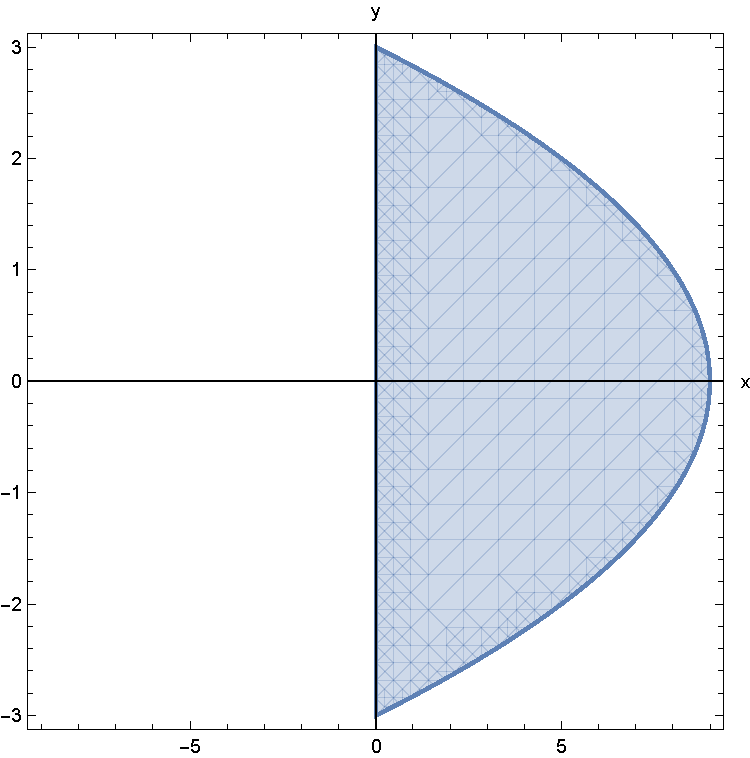
\includegraphics[scale=0.5]{p7.pdf}
\end{center}
It is bounded to the left by the $y$-axis, and to the right by the parabola $x=9-y^2$. The value of the area is
\begin{align*}
\int_{-3}^{3} \int_{0}^{9-y^2} \, dx\, dx & = \int_{-3}^{3}\left[ x \Big|_{x=0}^{x=9-y^2} \right] \, dy \\
& = \int_{-3}^{3} (9-y^2) \, dx \\
& = 9y-\frac{y^3}{3} \Big|_{y=-3}^{y=3}\\
& = 36
\end{align*}
\end{newsolution}

\begin{exercise}{8}
Use a double integral to find the volume of the tetrahedron bounded by the xy, xz, yz planes and the plane given by the equation 
\begin{equation*}
x+y+z=2.
\end{equation*}
\end{exercise}

\begin{newsolution}
A similar problem was solved in class. The key point here is to understand and parametrize the region of integration, in this case a triangle in the $xy$-plane, with vertices $(0,0,0)$, $(2,0,0)$, $(0,2,0)$. As such, we can compute the volume by means of the integral 
\begin{align*}
\int_{0}^{2} \int_{0}^{2-x} (2-x-y)\, dy \, dx & = \int_{0}^{2} \left[ 2y-xy-\frac{y^2}{2} \Big|_{y=0}^{y=2-x} \right] \, dx \\
& = \int_{0}^{2} \left[ 2(2-x)-x(2-x)-\frac{(2-x)^2}{2}\right] \, dx\\
& = \int_{0}^{2} \left[2 -2x +\frac{x^2}{2} \right] \, dx \\
& = \left[ 2x -x^2 + \frac{x^3}{6} \Big|_{x=0}^{x=2}\right] \\
& = \frac{4}{3}
\end{align*}

\end{newsolution}

\begin{exercise}{9}
Evaluate the iterated integral
\begin{equation*}
 \int_{0}^{4} \int_{0}^{\sqrt{16-y^2}} (x^2+y^2) \, dx \, dy
\end{equation*}
by converting it to polar coordinates.
\end{exercise}

\begin{newsolution}
Below is a plot of the region of integration, 
\begin{center}
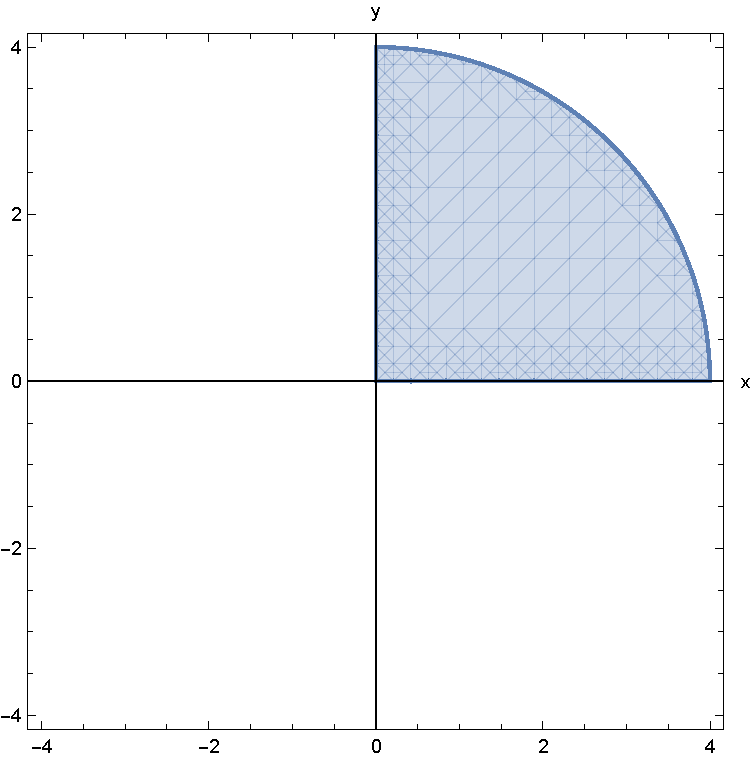
\includegraphics[scale=0.5]{p8.pdf}
\end{center}
This region can be parametrized in polar coordinates by: $0 \leq r \leq 4$, $0 \leq \theta \leq \frac{\pi}{2}$. Thus the integral can be written as 
\begin{align*}
\int_{0}^{4} \int_{0}^{\sqrt{16-y^2}} (x^2+y^2) \, dx \, dy & = \int_{0}^{\frac{\pi}{2}}\int_{0}^{4} (r^2) r\, dr \, d\theta \\
& = \int_{0}^{\frac{\pi}{2}} \left[ \frac{r^4}{4} \Big|_{r=0}^{r=4} \right] \, d\theta \\
& = \int_{0}^{\frac{\pi}{2}} 64 \, d\theta \\
& = 32\pi.
\end{align*}
\end{newsolution}

\begin{exercise}{10} 
Use a double integral to find the area of the region bounded by the equation 
\begin{equation*}
 r= 2\sin(2\theta).
 \end{equation*}
\end{exercise}

\begin{newsolution}
A plot of the curve (following the convention announced explained in the supplemental course notes on polar coordinates) is outlined below.
\begin{center}
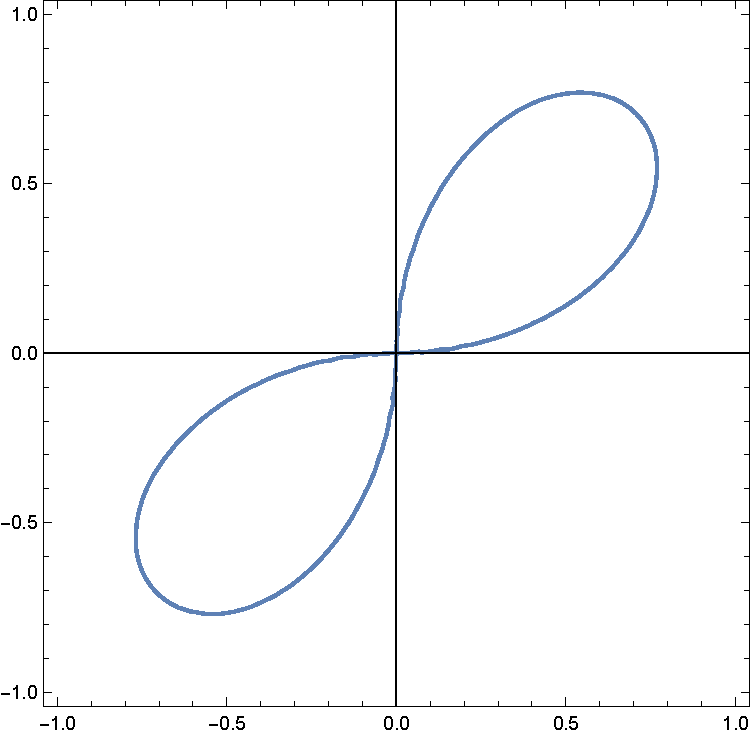
\includegraphics[scale=0.4]{polar_p6.pdf}
\end{center}
This curve is defined for $\theta \in \left[0,\frac{\pi}{2}\right] \cup \left[\pi, \frac{3\pi}{2}\right]$. 
By means of symmetry, we may describe the area of the region enclosed by this curve as twice the area of the petal in the first quadrant, that is,
\begin{align*}
\mathrm{Area} & = 2 \int_{0}^{\frac{\pi}{2}} \int_{0}^{2\sin(2\theta)} r\, dr \, d\theta \\
& = 2\int_{0}^{\frac{\pi}{2}} \left[ \frac{r^2}{2} \Big|_{r=0}^{r=2\sin(2\theta)} \right] \, d\theta \\
& = \int_{0}^{\frac{\pi}{2}} 4\sin^2(2\theta) \, d\theta \\
& = \int_{0}^{\frac{\pi}{2}}2(1-\cos(4\theta))d\theta \\
& = \left[2\theta -2\sin(4\theta) \Big|_{\theta = 0}^{\theta = \frac{\pi}{2}} \right] \\
& = \pi.
\end{align*}
\end{newsolution}

\end{document}

